\setcounter{chapter}{1}
\chapter{Sistemi Dinamici}

\section{Equazioni Differenziali Ordinarie}

Un equazione differenziale ordinaria \`{e} una funzione F che mette in relazione $\bm{x}(t)$ dipendente dal tempo alle sue derivate successive.
\begin{equation}
	F(\bm{x}(t),\dot{\bm{x}}(t),...,\bm{x}^{n}(t)) = 0
\end{equation}

\begin{definition}
	Definiamo una EDO (equazione differenziale ordinaria) di ordine n-simo in base al grado massimo di derivazione che compare nell'equazione.
\end{definition}
\begin{definition}
	Se la relazione 2.1 \`{e} esplicitabile rispetto alla derivata di ordine massimo, allora la EDO ottenuta si dice che \`{e} in \textbf{forma normale}
\begin{equation}
	\bm{x}^{n} = f(\bm{x}(t),\dot{\bm{x}}(t),...,\bm{x}^{n-1}(t))
\end{equation}
\end{definition}

\noindent Risolvere un equazione differenziale vuol dire determinare $\bm{x}(t)$ tale per cui la relazione 2.1 sia soddisfatta. Al procedimento di risoluzione dell'equazione si da il nome di \textbf{integrazione}.

\begin{theorem}
	Data un equazione differenziale del secondo ordine esprimibile in forma normale
	\begin{equation*}
		\ddot{x} = f(x,\dot{x})
	\end{equation*}
essa \`{e} sempre esprimibile come sistema di equazione differenziali del primo ordine
\begin{equation*}
	\left \{ \begin{array}{l}
		\dot{x} = y \\
		\dot{y} = f(x,y,t)
	\end{array} \right. 
\end{equation*}
\end{theorem}
\begin{remark} In realt\`{a} questo teorema \`{e} valido per EDO di qualsiasi ordine n, ma ai fini del capitolo non compariranno equazioni di ordine superiore al secondo.	
\end{remark}

\begin{theorem}[\textbf{Teorema di esistenza e unicit\`{a}}]
Si consideri il seguente sistema che prende il nome di problema di Cauchy, costituito da EDO al primo ordine e condizioni iniziali $\bm{x}(t_0) = \bm{x}_0$
\begin{equation*}
	\left \{ \begin{array}{l}
		\dot{\bm{x}} = F (\bm{x},t) \\
		\bm{x}(t_0) = \bm{x}_0
	\end{array}\right.
\end{equation*}	
Se F soddisfa le seguenti condizioni in intorno U di $\bm{x}_0$:
\begin{itemize}
	\item coninuit\`{a} rispetto t $\in I$.
	\item pi\`{u} della continuit\`{a} rispetto $\bm{x}$ e $\bm{\dot{x}}$.
\end{itemize}
allora il problema di Cauchy ammette una e una sola definizione definita in un aperto $(t_0 - \delta,t_0 + \delta)$.
\end{theorem}

\subsubsection{Esempio}

Prendiamo il seguente problema di Cauchy 
\begin{equation*}
	\left \{ \begin{array}{l}
		\dot{x} = \sqrt{|x|}\\
		x(0) = 0
	\end{array} \right.
\end{equation*}
la funzione $f(x) = \sqrt{|x|}$ ha un punto di discontinuit\`{a} in x = 0, infatti si ha un punto di cuspide. Di conseguenza in un intorno $(-\delta,\delta)$ di $t_0 = 0$ si hanno due soluzioni coincidenti nel punto x = 0.

\begin{remark}
Il numero di condizioni iniziali necessarie \`{e} dato dal prodotto del numero delle variabili indipendenti e dimensione dello spazio vettoriale.
Per esempio se prendiamo $\bm{x} \in \mathbb{R}^{3}$, abbiamo $dim(\mathbb{R}^{3}) = 3$, e le variabili indipendenti sono $\bm{x},\bm{\dot{x}}$, complessivamente avremo bisogno di $3 \times 2 = 6$ condizioni iniziali.	
\end{remark}

\subsection{Risoluzione di una EDO per quadrature}

Con risoluzione di un equazione differenziale per quadrature, si intende la determinazione di una soluzione utilizzando il calcolo integrale.
Possiamo definire due tipi di EDO al primo ordine risolubili con questa tecnica:
\begin{itemize}
	\item EDO esplicitamente dipendenti dal tempo $\dot{x} = f(t)$
	\item EDO autonome, ovvero $\dot{x} = f(x)$
\end{itemize}

\subsubsection{EDO dipendenti esplicitamente dal tempo}
Se x(t) \'{e} una soluzione dell'equazione 
\begin{equation}
	\dot{x} = f(t)
\end{equation}
in un punto $(t_0,x_0)$ si ha che la pendenza della retta tangente a tale punto \`{e} data a $f(t_0)$. Senza l'utilizzo di operazioni algebriche possiamo studiare il comportamento della funzione f(t) e delineare un comportamento della soluzione.

\noindent Nel caso della funzione f(t), abbiamo che fissato un valore $\overline{t}$ tutte le funzioni della forma $x(\overline{t}) + k \; \forall k \in \mathbb{R}$ sono soluzione dell'equazione differenziale 2.3. Di conseguenza possiamo definire per una soluzione le seguenti propriet\`{a}:
\begin{itemize}
	\item traslando una soluzione verticalmente si ottengono le altre.
	\item fissato un valore $t_0$ arbitrario, la famiglia delle soluzioni viene parametrizzata da $x_0$.
\end{itemize}
L'ultima propriet\`{a} discende dal fatto che determinare una soluzione dell'equazione 2.3 coincide nel determinare una primitiva della funzione f(t), ovvero
\begin{equation*}
	\int_{x_0}^x d\xi = \int_{t_0}^t f(\tau)d\tau
\end{equation*}
che equivale a 
\begin{equation*}
	x = x_0 + \int_{t_0}^{t} f(\tau) d\tau 
\end{equation*}
e prende il nome di soluzione per quadrature.

\subsubsection{EDO autonome}
Consideriamo un sistema autonomo descritto dall'equazione 
\begin{equation}
	\dot{x} = f(x)
\end{equation}
dove il secondo membro non dipende esplicitamente dal tempo, ma ne dipende solo implicitamente. Qualitativamente si osserva che le rette tangenti sono invarianti per traslazione lungo la direzione orizzontale. Anche in questo caso vogliamo determinare $x(t)$ che sia soluzione di 2.4. Osserviamo che se x(t) \`{e} soluzione anche $x_1(t-t^{\prime}) \; \forall t^{\prime} \in \mathbb{R}$ lo \`{e}. 
\subsubsection{Esempio}
Si consideri il seguente problema di Cauchy
\begin{equation*}
	\left \{ \begin{array}{l}
		\frac{dx}{dt} = 3x^{\frac{2}{3}} \\[0.2in]
		x(0) = x_0
	\end{array} \right.
\end{equation*}
dove $f(x) = 3x^{\frac{2}{3}}$ \`{e} una equazione differenziale autonoma. Osserviamo che la derivata prima di f(x) possiede un punto di cuspide in x=0. Risolvedo il l'equazione per quadrature otteniamo
\begin{equation*}
	\int \frac{dx}{3x^{\frac{2}{3}}} = \int dt \Rightarrow x(t) = (t+c)^3
\end{equation*}
per determinare la  costante c d'integrazione imponiamo le condizioni iniziali 
\begin{equation*}
	x(0) = c^3 \Rightarrow c = x_0^{\frac{1}{3}}
\end{equation*}
e dunque 
\begin{equation*}
	x(t) = (t + x_{0}^{\frac{1}{3}})^{3}
\end{equation*}
Tale soluzione \`{e} unica se $x_0 \neq 0$. Infatti nel caso in cui $x_0 = 0 $ si ha che $x(t) = t^3$ \`{e} soluzione del problema di Cauchy, ma anche x(t) = 0 \`{e} soluzione $\forall t \in \mathbb{R}$. Quindi non si ha pi\`{u} l'unicit\`{a} della soluzione dato che per t=0 le due soluzioni coincidono.

\subsection{EDO del primo ordine a variabili separabili}

Presa una EDO del primo ordine della forma 
\begin{equation}
	\dot{x} = f(x,t)
\end{equation}
la cui funzione \`{e} esprimibile come $f(x,t) = g(x)h(t)$, dove g(x) e h(t) sono $\neq 0$ in un intorno aperto di un tempo $t_0$ si avr\`{a} che l'equazione differenziale 2.5 \`{e} risolubile per separazione riscrivendola come 
\begin{equation}
	\int_{x_0}^{x} \frac{d\xi}{g(\xi)} = \int_{t_0}^t h(\tau)d\tau
\end{equation}
e la cui soluzione \`{e} data dalle primitive G(x) e H(t) 
\begin{equation*}
	G(x) = H(t) +c
\end{equation*}
dove c \`{e} una costante e viene definita dalla condizioni iniziali del problema.


\section{Oscillatori Armonici}

\subsection{Oscillatore Armonico Semplice}

Dato un sistema isolato, costituito da una punto materiale di massa \textit{m} su cui agisce una forza elastica di costante k vincolata a muoversi lungo una sola direzione, abbiamo che l'equazione dinamica \`{e} descritta da 
\begin{equation*}
	F = \pm kx 
\end{equation*}
che equivale ad un equazione differenziale del secondo ordine della forma 
\begin{equation}
	\ddot{x} \pm \frac{k}{m}x = 0
\end{equation}
posto $\frac{k}{m} = \omega^2$ possiamo determinare il polinomio caratteristico associato all'equazione rispetto agli autovalori $\lambda$
\begin{equation}
	P(\lambda) = \lambda^2 \pm \omega^2 = 0
\end{equation}
Nel caso negativo 
\begin{equation*}
	\lambda^2 - \omega^2 = 0 \Rightarrow \lambda_{1} = \omega \quad \text{e} \quad \lambda_2 = - \omega 
\end{equation*}
la soluzione dell'equazione \`{e} data dalla combinazione lineare
\begin{equation}
	x(t) = K_1 \;e^{\omega t} + K_2 \; e^{-\omega t} \equiv K_1 \; Cosh(\omega t) + K_2 \; Sinh(\omega t)
\end{equation}
dove per $\omega > 0 $ e valori generici di $K_1$ e $K_2$ diversi da zero si ha che $|x(t)| \rightarrow \infty$ per $t \rightarrow \pm \infty $.\newline
\\
Ne caso positivo 
\begin{equation*}
	\lambda^2 + \omega^2 = 0 \Rightarrow \lambda_{1} = i\omega \quad \text{e} \quad \lambda_2 = -i\omega 
\end{equation*}
e la soluzione della forma 
\begin{equation}
	x(t) = A \; \cos(\omega t) + B \; \sin(\omega t) \equiv K \cos(\omega t + \phi)
\end{equation}
per $K = \sqrt{A^2 + B^2}$, $A = \cos{\phi}$ e $B = \sin \phi$

\subsection{Oscillatore Armonico Smorzato}

Si ipotizzi di avere un sistema isolato come nella trattazione precedente, ma oltre alla forza elastica, agisce anche una forza di attrito viscoso. l'equazione che fornisce una descrizione della dinamica secondo la fisica Newtoniana \`{e} data dalla relazione
\begin{equation*}
	F = -kx - \eta \dot{x}
\end{equation*}
che equivale all'equazione differenziale ordinaria del secondo ordine 
\begin{equation}
	\ddot{x} + 2\gamma\dot{x} + \omega^2x = 0 
\end{equation}
dove $2\gamma = \frac{\eta}{m}$. Il polinomio caratteristico associato coincide con un equazione di secondo grado 
\begin{equation*}
	\lambda^2 + 2 \gamma \lambda + \omega^2 = 0
\end{equation*}
che ammette soluzione in $\lambda$
\begin{equation*}
	\lambda_{\pm} = -\gamma \pm \sqrt{\gamma^2-\omega^2}
\end{equation*}
dove $|\gamma| < |\omega|$ e $i \Omega = \gamma^2 - \omega^2 \geq 0$. La soluzione di 2.11 \`{e} della forma 
\begin{equation}
	x(t) = e^{-\gamma t} \left [ A \cos (\Omega t) + B \sin (\Omega t) \right ] \equiv Ke^{-\gamma t}\cos(\Omega t + \phi) 
\end{equation} 

 
\begin{figure}[ht]
\vspace{0.1in}
\includegraphics[width = 12cm]{damped}	
\centering
\vspace{0.2in}
\caption{Soluzione dell'oscillatore armonico smorzato}
\end{figure}

\subsection{Oscillatore armonico forzato}
Si immagini di avere un sistema isolato, in cui agiscono una forza elastica di costante k e un forza periodica $F = A \cos(bt)$. L'equazione dinamica descritta dalle leggi di Newton \`{e} data da 
\begin{equation}
	F = -kx + A \cos(bt)
\end{equation}
e l'equazione differenziale associata \`{e} della forma 
\begin{equation}
	\ddot{x} + \omega^2x = A \cos (bt)
\end{equation}
ovvero una EDO del secondo ordine non omogenea. Per un equazione lineare una soluzione \`{e} data dalla somma di una soluzione $x_O$ qualsiasi dell'equazione omogenea e di una soluzione particolare $x_P$.
\begin{equation*}
	x(t) = x_O + x_P
\end{equation*}
L'equazione omogenea coincide con quella dell'oscillatore armonico semplice di conseguenza 
\begin{equation*}
	x_O = K_1 \cos(\omega t) + K_2 \sin(\omega t)
\end{equation*}
Per determinare la soluzione particolare usiamo un approccio euristico, ovvero partendo da un guess della soluzione 
\begin{equation*}
	x_P = \mu \cos(b t)
\end{equation*}
Sostituendo nell'equazione 2.14 si determina il valore di $\mu$
\begin{equation*}
	\mu(\omega^2 - b^2) \cos(bt) = A \cos(bt) \Rightarrow A  = \mu (\omega^2 - b^2) \Rightarrow
\boxed{\mu = \frac{A}{(\omega^2 - b^2)}}
\end{equation*}
Se la frequenza b della forzante non coincide con quella propria del sistema $\omega$, ovvero $b \neq \omega$, $\mu$ \`{e}  finito. La soluzione del sistema \`{e} 
\begin{equation}
	x(t) = K_1 \cos(\omega t) + K_2 \sin(\omega t) + \frac{A}{(\omega^2 - b^2)} \cos (bt)
\end{equation}
Quando il rapporto tra b e $\omega $ non \`{e} un multiplo razionale di $\pi$, $\dot{x}(t)$ non \`{e} periodica, ma solo limitata.\newline

\noindent Se ipotizziamo che all'interno del sistema sia presente anche una forza di attrito viscoso, il procedimento risolutivo \`{e} analogo per la determinazione della soluzione particolare. Cambia solo la soluzione dell'equazione omogenea in cui compare un termine $e^{- \gamma t}$. 

\noindent Quando si ha una un sistema di questo tipo, dopo un transiente il sistema di mette sulla frequenza della forzante e per tempi sufficientemente lunghi la soluzione \`{e} asintotica alla soluzione particolare.

\subsubsection{Che cosa succede se frequenza propria del sistema e frequenza della forzante coincidono ?}
L'equazione differenziale coincide con quella espressa in  2.14 solo che il termine $b = \omega $. Per risolvere l'equazione 
\begin{equation}
	\ddot{x} + \omega^2 x= A\cos(\omega t) 
\end{equation}
si usa il metodo delle \textit{variazione delle costanti arbitrarie}, ovvero si considera un ansatz della forma $x_P = H(t) \sin(\omega t)$ e lo si sostituisce nell'equazione 2.16.
\begin{equation}
	\ddot{k} \sin(\omega t) - 2k\omega \cos(\omega t) = A \cos(\omega t)
\end{equation}
Ottenendo un equazione diferenziale del secondo ordine rispetto a \textit{k(t)}. Che possiamo risolvere come 
\begin{equation*}
	\left \{ \begin{array}{l}
		\ddot{k} = 0 \\ 
		\dot{k} = \frac{A}{2\omega} 
	\end{array} \right. 
	\Rightarrow k(t) = \frac{A}{2\omega} \;t + c
\end{equation*}
dove la seconda equazione \`{e} stata risolta per quadrature. In conclusione la soluzione \`{e} data da 
\begin{equation}
	x(t) = \frac{A t}{2 \omega} \cos(\omega t)
\end{equation}
Quando si inserisce una forzante con la stessa frequenza propria del sistema, le oscillazioni aumentato d'ampiezza.

\section{Sistemi Newtoniani conservativi nel piano}

Nella sezione precedente si sono introdotte alcuni metodi risolutivi per alcune categorie di equazioni differenziali, ma non sempre \`{e} possibile ottenere una soluzione esplicita. Per questo motivo si procede con un analisi qualitativa del comportamento del sistema e delle sue soluzioni.
\newpage 
\subsection{Sistema Dinamico nel piano }

Consideriamo un punto materiale, il cui moto avviene nel piano. La sua posizione in ogni istante di tempo $t \in \mathbb{R}$ sar\`{a} descritta dal vettore posizione
\begin{equation}
	\bm{r}(t) = \left [ x(t),y(t) \right ]
\end{equation}
che rappresenta una parametrizzazione di una curva C nel piano (x,y)
\begin{equation*}
	\bm{r} : \mathbb{R} \rightarrow \mathbb{R}^2
\end{equation*}
La derivata prima del vettore posizione $\bm{\dot{r}}(t)$  \`{e} data da 
\begin{equation*}
	\bm{\dot{r}}(t) = \lim_{h \rightarrow 0} \left [\begin{array}{c}
		\frac{x(t_0 +h) - x(t_0)}{h} \\[0.1in]
		\frac{y(t_0 + h) - y(t_0)}{h}
	\end{array} \right ]
\end{equation*}
e rappresenta geometricamente il vettore tange alla curva C.

\begin{definition}
	Diremo che la funzione $\bm{r}(t)$ \`{e} una parametrizzazione regolare (o liscia) della curva C se la sua derivata prima $\bm{\dot{r}}(t)  \neq 0 \; \forall \,t \in \mathbb{R}$.
\end{definition}

\begin{definition}
Dato un campo vettoriale $\vec{V}(x,y) = f(x,y) \bm{u}_{x} +g(x,y)\bm{u}_{y}$ diremo che una curva $\bm{r}(t)$ \`{e} una \textit{linea di flusso} di $\vec{V}$ se 
\begin{equation}
	\left \{ \begin{array}{l}
		\dot{x}(t) = f(x,y)\\
		\dot{y}(t) = g(x,y)
	\end{array} \right. 
\end{equation}
\end{definition}
\noindent Per determinare le linee di flusso bisogna determinare (x(t),y(t)) soluzione del sistema di EDO del primo ordine.


\begin{definition}
	Chiameremo sistema dinamico a un grado di libert\`{a} un sistema descritto dall'equazione differenziale
	\begin{equation}
		\ddot{x} = f(x) \quad \forall x \in \mathbb{R}
	\end{equation}
	\newpage 
che \`{e} equivalente al sistema di equazioni differenziale del primo ordine
\begin{equation*}
	\left \{ \begin{array}{l}
		\dot{x} = y \\
		\dot{y} = f(x)
	\end{array} \right.  \quad \forall x \in \mathbb{R}
\end{equation*}
\end{definition}

Si chiama \textbf{energia cinetica} la forma quadratica 
\begin{equation*}
	T = \frac{1}{2} \dot{x}^2
\end{equation*}

Si chiama \textbf{energia potenziale} la funzione 
\begin{equation*}
	U(x) = - \int_{x_0}^{x} f(\xi) d \xi
\end{equation*} 
Per la definizione che abbiamo dato dell'energia potenziale, abbiamo che U \`{e} la primitiva della funzione $f(\xi)$  di conseguenza $f(x) = - \frac{dU(x)}{dx}$ e quindi il sistema 2.21 possiamo riscriverlo come
\begin{equation}
		\left \{ \begin{array}{l}
		\dot{x} = y \\
		\dot{y} = - \frac{dU(x)}{dx}
	\end{array} \right.  \quad \forall x \in \mathbb{R}
\end{equation}

Si chiama \textbf{energia totale} la somma 
\begin{equation*}
	E = T + U
\end{equation*}
in questo modo l'energia totale \`{e} una funzione $E(x,\dot{x})$.

\begin{theorem}[\textbf{Legge della conservazione dell'energia}] L'energia totale di un punto materiale che si muove secondo l'equazione differenziale 2.21 si conserva: $ E(x,\dot{x}) $ non dipende da t.	
\end{theorem}

\begin{proof}
\begin{equation*}
	\frac{d (T+U)}{dt} = \dot{x} \ddot{x} + \frac{dU}{dx}\dot{x} = \dot{x}[\ddot{x} - f(x)] = 0 
\end{equation*}
\end{proof}

\noindent La conservazione dell'energia cinetica coincide nell'identificare delle curve si livello della funzione $E(x,\dot{x})$. Inoltre se tale teorema non \`{e} verificato un sistema della forma 2.22 non ammette soluzioni.

\begin{definition}
	Definiamo \textbf{variabile dinamica} una funzione
	\begin{equation*}
		W(x,y) : \Omega \subset \mathbb{R}^2 \rightarrow \mathbb{R}
	\end{equation*}
	per il sistema 2.20. Dove [x(t),y(t)] per $t \in [a,b]$ sono funzioni del tempo. Tale funzione \`{e} una parametrizzazione delle curve di livello del sistema.
\end{definition}

\begin{definition}
	Una variabile dinamica W(x,y) \`{e} detta costante del moto del sistema 2.20 se per ogni soluzione (x(t),y(t)), del sistema per $t \in [a,b]$ si ha che $W(x,y) = \text{costante}$ per $t \in [a,b]$.
\end{definition}
\subsection{Piano delle Fasi ad una dimensione}
 Consideriamo un piano con coordinate x,y. Questo piano prende il nome di \textbf{piano delle fasi}. I punti del piano delle fasi si dicono \textbf{punti di fase}. La parte destra del sistema associato all'equazione 2.21 definisce un campo vettoriale e prende il nome di \textbf{campo vettoriale delle velocit\`{a} di fase}. Abbiamo visto che la soluzione del sistema \`{e} data da $\bm{r}(t)$ che coincide con la parametrizzazione di una curva nel piano e nel piano delle fasi prende il nome di \textbf{curva di fase}. Che \`{e} data dalle rappresentazioni parametriche 
\begin{equation}
	x = \varphi(t) \quad y = \dot{\varphi}(t)
\end{equation}
Il moto del sistema sar\`{a} descritto da un punto che si muove lungo una curva del piano. La velocit\`{a} di fase data dal secondo termine in 2.23 \`{e} descritta dal punto stesso. L'insieme dei vettori delle velocit\`{a} definisce un campo vettoriale nel piano delle fasi e definisce l'equazione differenziale del processo.
\newpage 
\begin{figure}[!ht]
\vspace{0.2in}
\includegraphics[width = 7cm]{fasi}	
\centering
\vspace{0.2in}
\caption{Esempio di piano delle fasi}
\end{figure}

\section{Studio Qualitativo di un Sistema Dinamico Newtoniano Conservativo }

Consideriamo il sistema dinamico 
\begin{equation}
		\left \{ \begin{array}{l}
		\dot{x} = y \\
		\dot{y} = - \frac{dU(x)}{dx}
	\end{array} \right.  \quad \forall x \in \mathbb{R}
\end{equation}
 e prendiamo come variabile dinamica la funzione 
 \begin{equation*}
 	E(x,y) = \frac{1}{2}y^2+ U(x)
 \end{equation*}
che \`{e} una costante del moto, ovvero per ogni tempo t la funzione \`{e} costante e definisce una curva di livello nel piano delle fasi. Se si vuole avere un'idea del grafico dell'energia \`{e} sufficiente osservare che per y=0, nel piano (x,z) si definisce il grafico di U(x). Analogamente per $\overline{x}$ fissato si ha l'equazione di una parabola $E(\overline{x},y) = \frac{1}{2}y^2 + c$. Facendo scorrere il vertice della parabola lungo U(x) otteniamo il grafico di E(x,y). \newline
I livelli di energia che definiscono  le curve di livello sono simmetrie rispetto l'asse delle ordinate.

\begin{definition}
	Sia $\overline{x}$ tale che $U^{\prime}(\overline{x}) = 0$, allora il punto di fase $(\overline{x},0)$ \`{e} un punto di equilibrio per il sistema dinamico 2.24. Tale punto \`{e} classificabile come:
	\begin{itemize}
		\item \textbf{Stabile} se $U^{\prime \prime} (\overline{x}) > 0$. Date delle condizioni iniziali vicine al punto di equilibrio la soluzione rimane in un suo intorno.
		\item \textbf{Instabile} se $U^{\prime \prime} (\overline{x}) < 0$. Prese delle condizioni iniziali vicine a $\overline{x}$ la soluzione si allontana dal punto.
	\end{itemize}
\end{definition}

\subsubsection{Soluzioni ammesse per l'energia fissata}

Per un SDNC, fissata l'energia totale del sistema si ha che $E_0 = \frac{1}{2}y^2 + U(x)$ e dunque le soluzioni sono date da $y = \pm \sqrt{2(E_0 - U(x)}$ studiando il dominio di definizione, affinch\`{e} esistano delle soluzioni reali \`{e} necessario che $U(x) \leq E_0$.

\subsubsection{Esempio: Punto Materiale Libero}

Preso un punto materiale in movimento non soggetto a forze esterne il SDNC \`{e} dato da \
\begin{equation*}
	\left \{ \begin{array}{l}
		\dot{x} = y\\
		\dot{y} = 0
	\end{array} \right.
\end{equation*}
e l'energia totale del sistema \`{e} data da $E(x,y) = \frac{1}{2}y^2$. Osserviamo che:
\begin{itemize}
	\item Per $E_0 < 0 $ non sono ammesse soluzioni.
	\item Per $E_0 = 0 $ si hanno soluzioni stazionarie (x,0) $\forall x \in \mathbb{R}$.
	\item Per $E_0 > 0$ si hanno moti compatibili la cui soluzione del sistema coincide con $y = \pm\sqrt{2E_0}$ ed $\forall x \in \mathbb{R}$. Il segno di y stabilisce il senso di percorrenza della particella.
\end{itemize}

 
\begin{figure}[!ht]
\vspace{0.1in}
\includegraphics[width = 10cm]{free_motion}	
\centering
\vspace{0.1in}
\caption{Piano delle fasi del sistema dinamico}
\end{figure}

\newpage

\subsubsection{Esempio : Caduta dei Gravi}

Si consideri un punto materiale soggetto alla forza di attrazione gravitazione F = mg, il potenziale associato \`{e} dato da U = gx per m=1. Il sistema dinamico associato \`{e} dato dalle equazioni 
\begin{equation*}
	\left \{ \begin{array}{l}
		\dot{x} = y \\
		\dot{y} = -g 
	\end{array} \right.
\end{equation*}
l'energia totale del sistema \`{e} data da $E = \frac{1}{2} y^2 + gx$.

\begin{figure}[!ht]
\vspace{0.1in}
\includegraphics[width = 10cm]{gravity}	
\centering
\vspace{0.1in}
\caption{Piano delle fasi del sistema dinamico}
\end{figure}

I punti d'inversione del moto sono dati da  y = 0, per un energia $E_0$ fissata si ha che $x = -\frac{E_0}{g}$. I punti d'inversione hanno tangente verticale, poich\`{e} data la soluzione 
\begin{equation*}
	y = \pm \sqrt{2(E_0 + gx)}
\end{equation*}
si ha che
\begin{equation*}
	y^{\prime} = \pm \frac{g}{2 \sqrt{2(E_{0} +gx)}} 
\end{equation*}
che per $x = -\frac{E_0}{g}$ si ha $y^{\prime} = \pm \infty $. \newline
Come si comportano le curve di fase x(t) per $t \rightarrow \pm \infty $?
\begin{equation*}
	y = \pm \sqrt{2(E_0 + gx)} \approx  \pm \sqrt{2}\sqrt{\vert x \vert } \rightarrow \pm \infty 
\end{equation*}
Non sono presenti punti di equilibrio in quanto la derivata del potenziale non si annulla mai.



\subsubsection{Esempio : Oscillatore Armonico}

Data una particella soggetta ad una forza elastica F = -kx, il potenziale associato \`{e} dato da U(x) = $\frac{1}{2}kx^2$. Il sistema dinamico \`{e} descritto dalle equazioni
\begin{equation*}
	\left \{ \begin{array}{l}
		\dot{x} = y \\
		\dot{y} = -kx 
	\end{array} \right.
\end{equation*}
L'energia totale $E = \frac{1}{2}y^2 + \frac{1}{2}kx^2$ \`{e} definita sempre positiva e dunque non esistono soluzioni per $E_0 < 0$. Il punto (0,0) definisce un punto di equilibrio stabile nel piano delle fasi. Le curve di livello data da valori fissati dell'energia descrivono delle curve chiuse nel piano, schiacciate rispetto al punto di minimo. Nei punti d'inversione y=0 (dove la velocit\`{a} si annulla) il campo ha tangenza verticale, con segno negativo nel semipiano positivo e segno positivo in quello negativo.
\begin{figure}
\centering
\begin{minipage}{.5\textwidth}
  \centering
  \includegraphics[width= 1\linewidth]{harmo}
  \captionof{figure}{Piano delle fasi dell'oscillatore armonico}
  \label{fig:test1}
\end{minipage}%
\begin{minipage}{.5\textwidth}
  \centering
  \includegraphics[width= 0.8\linewidth]{Oscill}
  \captionof{figure}{Potenziale elastico}
  \label{fig:test2}
\end{minipage}
\end{figure}

\subsection{Rette Separatici}

Si consideri un punto di equilibrio $(\underline{x},0)$ instabile, ovvero $\overline{x}$ \`{e} un punto di massimo per l'energia potenziale U(x). In tale punto la curva \`{e} composta da pi\`{u} traiettorie e  viene definita separatrice l'equazione
\begin{equation}
	y = \pm \sqrt{\vert U^{\prime \prime}(x) \vert}(x-\underline{x})
\end{equation}

\begin{proof}
	Sviluppiamo con Taylor l'energia potenziale fino al secondo ordine in un intorno del punto di equilibrio
	\begin{equation*}
		U(x) \approx U(\overline{x}) + U^{\prime}(\overline{x})(x-\overline{x})+\frac{1}{2}U^{\prime \prime}(\overline{x})(x-\overline{x})^2
	\end{equation*}
sostituendo nell'equazione dell'energia totale del sistema per un suo valore fissato $E_0$ si ha che 
\begin{equation*}
	\left  (y -\sqrt{\vert U^{\prime \prime}(x) \vert}(x-\overline{x})\right)\left (y +\sqrt{\vert U^{\prime \prime}(x) \vert}(x-\overline{x})\right) = 0
\end{equation*}
e dunque si ottiene 2.25.

\end{proof}

\subsection{Piccole Oscillazioni}

Si consideri un punto di equilibrio stabile $(\overline{x} ,0)$, ovvero un punto di minimo per l'energia potenziale U(x). Espandendo con Taylor in un intorno del punto abbiamo che 
\begin{equation*}
	U(x) \approx U(\overline{x}) + \frac{1}{2}U^{\prime \prime} (\overline{x})(x-\overline{x})^2
\end{equation*}
dove $U(\overline{x}) = E_0$. A meno di una costante in un intorno del punto di equilibrio, il potenziale si comporta nello stesso modo di un oscillatore armonico. Quindi la funzione nell'intorno \`{e} approssimabile come una parabola e di conseguenza le orbite sono curve chiuse e periodiche. Il periodo \`{e} dato da 
\begin{equation*}
	T = \frac{2 \pi}{\omega}  \quad \text{dove} \quad \omega =\sqrt{U^{\prime \prime}(x)} 
\end{equation*}
e quindi
\begin{equation}
	T = \frac{2 \pi}{\sqrt{U^{\prime \prime}(x)}}
\end{equation}

\subsection{Tempo di Percorrenza di una Traiettoria}
\begin{wrapfigure}{r}{0.5\textwidth}
\vspace{-0.3in}
  \begin{center}
    \includegraphics[width=0.48\textwidth]{period}
  \end{center}
\end{wrapfigure}

Supponiamo di voler determinare il tempo di percorrenza lungo un segmento di una traiettoria data da un energia totale $E_0$ fissata, partendo da un punto nel piano delle fasi $(x_a,v_a)$ e raggiungendo $(x_b,v_b)$. Sappiamo che una traiettoria \`{e} descritta dalla relazione 
\begin{equation*}
	y = \sqrt{2(E_0 - U(x))}
\end{equation*}
che possiamo riscrivere come 
\begin{equation*}
	\dot{x} = \sqrt{2(E_0 - U(x))}
\end{equation*}
\newpage
e procedendo per integrazione otteniamo
\begin{equation}
 \int_{t_a}^{t_b}dt = \int_{x_a}^{x_b} \frac{dx}{\sqrt{2(E_0 -U(x))}}
\end{equation}
Si osservi che l'integrale 2.27 non presenta problemi d'integrazione fin tanto che gli estremi rispetto alla posizione non coincidono con dei punti d'inversione, ovvero laddove U(x) = $E_0$.
\newline

\noindent \textbf{Che cosa succede nei punti d'inversione ?}
\newline

\noindent Consideriamo il limite per $x \rightarrow x_R$ dove $x_R$ \`{e} il primo punto d'inversione percorrendo la curva chiusa in senso orario.
\begin{equation}
	\lim_{x \rightarrow x_R} \Delta t = \lim_{x \rightarrow x_R} \int_{x_a}^{x} \frac{dx}{\sqrt{2(E_0 -U(x))}} 
\end{equation}
sviluppando con Taylor in un intorno di $x_R$ l'argomento della radice del denominatore 
\begin{equation*}
	2(E_0 -U(x)) \approx 2   [ E_0 - U(x_R) -\underbrace{U^{\prime}(x_R)}_{<  0}(x-x_R) ] = 2 \vert U^{\prime}(x_R)\vert (x-x_R)
\end{equation*}
l'equazione 2.28 diventa
\begin{equation*}
	T(x \rightarrow x_R) \approx \lim_{x \rightarrow x_R} \int_{x_a}^{x} \frac{dx}{\sqrt{2|U^{\prime}(x_R)| (x-x_R)}} \approx \lim_{x \rightarrow x_R} \int_{x_A}^{x} \frac{dx}{\sqrt{x}} < \infty 
\end{equation*} 
e quindi il tempo di percorrenza \`{e} finito.
Per un orbita chiusa il tempo di percorrenza di tutto il cammino \`{e}
\begin{equation}
	T = 2 \int_{x_L}^{x_R} \frac{dx}{\sqrt{2(E_0 -U(x))}}
\end{equation} 
dove gli estremi d'integrazione $x_L$ e $x_R$ sono rispettivamente il punto d'inversione sinistro e destro.
Come si \`{e} visto nelle sezioni precedenti esistono orbite che non sono cammini continui, ma hanno punti di separazione; possiamo ugualmente affermare che il tempo di percorrenza sia finito per questa classe di percorsi ?
\newpage 

\noindent \textbf{Come cambia il tempo per una curva separatrice ?}

\begin{wrapfigure}{l}{0.5\textwidth}
\vspace{-0.3in}
  \begin{center}
    \includegraphics[width=0.48\textwidth]{close}
  \end{center}
\end{wrapfigure}
\vspace{0.3in}
\noindent Consideriamo un cammino come nella figura adiacente, in cui \`{e} presente un punto di separazione $x_{P}$. In questo caso si hanno quattro cammini separati e non un unico percorso come nel caso dell'orbita chiusa. Tali configurazioni nel caso dei sistemi dinamici conservativi emergono per i punti di massimo dell'energia potenziale, ovvero $U^{\prime \prime}(x) < 0$. Per determinare il tempo di percorrenza della traiettoria da un punto di partenza $x_A$, procediamo a sviluppare con Taylor l'argomento della radice del denominatore dell'equazione 2.28 in un intorno di $x_P$. A differenza del caso precedente lo sviluppo si arresta al secondo ordine d'infinitesimo.
\begin{equation*}
	2(E_0 -U(x)) \approx 2   [ E_0 - U(x_R) -\underbrace{U^{\prime}(x_R)}_{ = 0}(x-x_R) - \frac{1}{2}\underbrace{U^{\prime \prime}(x_R)}_{ < 0}(x-x_R)^2 ] =
\end{equation*} 
\begin{equation*}
	= \vert U^{\prime \prime}(x_R) \vert (x-x_R)^2
\end{equation*}
l'equazione 2.28 diventa 
\begin{equation*}
	T  \approx \lim_{x \rightarrow x_P} \int_{x_A}^{x} \frac{dx}{\sqrt{|U^{\prime \prime}(x)|}|x-x_P|} = \frac{1}{\sqrt{\vert U^{\prime \prime}(x)}} 
	\lim_{x \rightarrow x_P}\int_{x_A}^{x} \frac{dx}{\vert x - x_P \vert} = 
\end{equation*}
\begin{equation*}
	= \frac{1}{\sqrt{\vert U^{\prime \prime}(x)}} 
	\lim_{x \rightarrow x_P}  [ \log(\vert x - x_P \vert ) ]_{x_A}^{x} = \lim_{x \rightarrow x_P} \log(\vert x - x_P \vert) + C \rightarrow \infty 
\end{equation*}
In conclusione una particella non raggiunge la posizione $x_P$ in un tempo finito.

\newpage

\subsection{Approssimazione di un periodo}

 
\begin{figure}[!ht]
\includegraphics[width = 9cm]{approx}	
\centering
\caption{Approssimazione del periodo per un punto di minimo}
\end{figure}

Si consideri un sistema dinamico Newtoniano e conservativo. Sia $x_0$ il punto di minimo del potenziale U(x) associato al sistema. Esistono casi di studio di un sistema in cui l'integrale 2.29 non \`{e} sempre risolvibile per un energia $\overline{E}$ fissata; in queste configurazioni per ottenere il valore del periodo lungo l'orbita si procede ad approssimarla scegliendo due funzioni  f(x) e g(x) tali per cui valgano le seguenti propriet\`{a}:
\begin{itemize}
	\item  $f(x) > U(x) \quad \forall x \in (x_L,x_R)$ 
	\item $g(x) < U(x) \quad \forall x \in (x_L,x_R)$
	\item $g(x_L) = U(x_L) =f(x_L)$ e $g(x_R) = U(x_R) = f(x_R)$
	\item $f(x) \leq  \overline{E} \quad \forall x \in [x_L,x_R]$ e dunque $g(x) \leq \overline{E}$
\end{itemize}

Poich\`{e} $g(x) \leq U(x) \leq f(x) \quad \forall x \in [x_L,x_R]$ abbiamo che $-g(x) \geq -U(x) \geq -f(x)$ e dunque 
\begin{equation*}
	2(\overline{E}  - g(x)) \geq 2(\overline{E} - U(x)) \geq 2(\overline{E}-f(x))
\end{equation*}
quindi possiamo stimare il periodo di una semi orbita chiusa come
\begin{equation*}
	\int_{x_L}^{x_R} \frac{dx}{\sqrt{2(E_0 -g(x))}} \leq \int_{x_L}^{x_R} \frac{dx}{\sqrt{2(E_0 -U(x))}} \leq \int_{x_L}^{x_R} \frac{dx}{\sqrt{2(E_0 -f(x))}}
\end{equation*}
Da un punto di vista operativo possiamo scegliere f(x) e g(x) come unione di spezzate che approssimano la funzione U(x).

\begin{wrapfigure}{r}{0.6\textwidth}
\vspace{-0.6in}
  \begin{center}
    \includegraphics[width=0.6\textwidth]{approx1}
  \end{center}
\end{wrapfigure}
\vspace{0.3in}
\noindent Se $U^{\prime \prime}(x) > 0 $ come nei casi considerati nelle figure di questa sezione possiamo definire f(x) considerando le rette secanti che passano per il punto d minimo $x_0$ del potenziale. Mentre per g(x) si usano le rette tangenti in $x_L$ e $x_R$ punti d'inversione e la costante orizzontale $U(x_0)$. Si procede in modo analogo nel caso in cui $U^{\prime \prime} (x) < 0$. 

\subsection{Diagramma di Biforcazione e dipendenza dei punti di equilibrio da un parametro}

Data una famiglia di potenziali dipendenti da un parametro $U_{\alpha}(x)$, vogliamo stabilire se la stabilit\`{a} di un punto di equilibrio appartenente a tale famiglia, cambia al variare del parametro $\alpha$. Prendiamo in considerazione un potenziale della forma 
\begin{equation}
	U_{\alpha}(x) = (x^2-\alpha)^2
\end{equation}
\newpage 

cerchiamo i punti critici del potenziale risolvendo l'equazione $U_{\alpha}^{\prime}(x) = 0$
\begin{equation*}
	4x(x^2 - \alpha)= 0 
\end{equation*}
trovando i punti $x_1 = 0 $ e $x_{2,3} = \pm \sqrt{\alpha}$. Nel piano delle fasi otteniamo i seguenti punti di equilibrio:
\begin{itemize}
	\item (0,0) esiste per ogni valore di $\alpha$ 
	\item $(\sqrt{\alpha},0)$ e $(-\sqrt{\alpha},0)$ per condizione di esistenza tali punti sono ammessi solo se $\alpha \geq 0$.
\end{itemize}
Studiando il segno della derivata seconda del potenziale determiniano la natura dei punti critici e di conseguenza la loro stabilit\`{a} nel piano delle fasi.
\begin{equation*}
	U^{\prime \prime}(x) = 0 
\end{equation*}
ottenendo
\begin{itemize}
	\item $U^{\prime \prime}(0) = - 4 \alpha $, dunque (0,0) \`{e} di equilibrio stabile se $\alpha <0$ e di equilibrio instabile per $\alpha > 0$
	\item $U^{\prime \prime}(\pm \sqrt{\alpha}) = 8\alpha$, quindi $(\pm\sqrt{\alpha},0)$ \`{e} stabile per $\alpha > 0$ dato che tali punti esistono solo per $\alpha \geq 0$.
\end{itemize}
Dato che i punti di equilibrio hanno $y = 0$ possiamo riassumere in grafico nel piano $(\alpha,x)$ le informazioni discusse nei punti precedenti. Tale grafico prende il nome di \textbf{diagramma di biforcazione}.

\begin{wrapfigure}{r}{0.5\textwidth}
\vspace{-0.4in}
  \begin{center}
    \includegraphics[width=0.5\textwidth]{bif}
  \end{center}
\end{wrapfigure}
\vspace{0.3in}
\noindent Per $x = \pm \sqrt{\alpha}$ si ha il grafico della radice quadrata rispetto ad $\alpha$. Con il tratto continuo si indica l'intervallo di valori $(-\infty, 0)$ rispetto al quale il punto (0,0) \`{e} di equilibrio stabile, mentre con quello tratteggiato l'intervallo di valori rispetto al quale \`{e} instabile.  
\newpage 

\begin{figure}[!ht]
\centering
\begin{minipage}{.5\textwidth}
  \centering
  \includegraphics[width= 1\linewidth]{poten1}
  \captionof{figure}{Potenziale per $\alpha < 0$}
  \end{minipage}%
\begin{minipage}{.5\textwidth}
  \centering
  \includegraphics[width=1\linewidth]{poten}
  \captionof{figure}{Potenziale per $\alpha > 0$}
\end{minipage}
\end{figure}
\begin{figure}[!ht]
\centering
\begin{minipage}{.5\textwidth}
  \centering
  \includegraphics[width= 1\linewidth]{potenphase1}
  \captionof{figure}{Piano fasi per $\alpha < 0$}
  \end{minipage}%
\begin{minipage}{.5\textwidth}
  \centering
  \includegraphics[width=1\linewidth]{potenphase}
  \captionof{figure}{Piano fasi per $\alpha > 0$}
\end{minipage}
\end{figure}

Dai grafici in figura osserviamo come cambia il grafico nel piano delle fasi al variare di $\alpha$. (0,0) da punto di equilibrio stabile per $\alpha <0$, diventa punto di equilibrio instabile  per $\alpha >0$ e si creano due buche di potenziale.

\section{Stabilit\`{a} Dei Sistemi Dinamici }

\begin{theorem}[\textbf{Teorema della scatola di flusso (o teorema di rettificazione dei campi vettoriali)}]
	Si consideri un sistema dinamico nel piano 
	\begin{equation*}
		\left \{ \begin{array}{l}
			\dot{x} = f(x,y) \\
			\dot{y} = g(x,y)
		\end{array} \right.
	\end{equation*}
e sia $(\tilde{x},\tilde{y})$ un punto non di equilibrio del sistema. Allora esiste un intorno B($\tilde{x},\tilde{y})$ e un opportuno cambio di coordinate (rettificazione)
\begin{equation*}
	\left [\begin{array}{c}
		r(x,y)\\
		s(x,y)
	\end{array} \right]
	: U \subset \mathbb{R}^2 \rightarrow \mathbb{R}^2
\end{equation*}
tale per cui il sistema dinamico di partenza \`{e} rappresentabile come 
\begin{equation*}
		\left \{ \begin{array}{l}
			\dot{r} = 0 \\
			\dot{s} = 1
		\end{array} \right.
	\end{equation*}
\end{theorem}
In sostanza il teorema ci dice che localmente possiamo sempre definire una trasformazione di coordinate tale per cui tutti i flussi sono laminari a patto che il punto non sia di equilibrio.

\subsubsection{Esempio}

Prendiamo il sistema dinamica dato da un oscillatore armonico con costante elastica k = 1.
\begin{equation*}
		\left \{ \begin{array}{l}
			\dot{x} = y \\
			\dot{y} = -x
		\end{array} \right.
\end{equation*}
utilizzando la parametrizzazione 
\begin{equation*}
		\left \{ \begin{array}{l}
			r = \sqrt{x^2+y^2} \\
			\dot{y} = \text{arctan}(\frac{y}{x})
		\end{array} \right.
\end{equation*}
preso un punto (x,y) lontano dal punto di equilibrio (0,0) si ha che vale il teorema di rettificazione
infatti
\begin{equation*}
	\dot{r} = \frac{\partial r}{\partial x}\frac{dx}{dt} + \frac{\partial r}{\partial y}\frac{dy}{dt} =\frac{2x}{2\sqrt{x^2+y^2}}\dot{x} + \frac{2y}{\sqrt{x^2+y^2}}\dot{y} = 0
\end{equation*}
e analogamente di dimostra che $\dot{s} = 1$.
\subsection{Stabilit\`{a} per Sistemi Lineari nel piano}

\begin{definition}
	Un punto di equilibrio $\tilde{\bm{x}}$ per il sistema dinamico $\bm{\dot{x}} = \bm{F}(\bm{x})$ \`{e} detto \textbf{stabile} secondo Lyapunov se $\forall \varepsilon > 0 \quad \exists \delta >0$  tale che l'evoluto temporale di un punto $\bm{x}_0 \in B_{\delta}(\bm{\tilde{x}})$ resta nell'insieme aperto $B_{\varepsilon}(\bm{\tilde{x}})$. Un punto di equilibrio che non \`{e} definito stabile secondo Lyapunov \`{e} definito \textbf{instabile}. 
\end{definition}

\noindent Un generico sistema lineare nel piano \`{e} una famiglia a quattro parametri 

\begin{equation}
	\left \{ \begin{array}{l}
		\dot{u} = au+bv\\
		\dot{v} = cu+dv
	\end{array} \right.
	\iff 
	\left [\begin{array}{c}
		\dot{u} \\
		\dot{v}
	\end{array} \right] =
	\underbrace{\left [ \begin{array}{cc}
		a & b \\
		c & d
	\end{array} \right]}_{ = A}
	\left [\begin{array}{c}
		u \\
		v
	\end{array} \right]
\end{equation}
\newline
dove u e v sono definite rispetto ad una base. Possiamo ricondurre il studio del sistema all'analisi della matrice associata. Gli autovalori possibili di A sono:
\begin{itemize}
	\item $\alpha \in \mathbb{R}$ distinti.
	\item $\alpha \in \mathbb{C}$ coniugati tra loro.
	\item $\alpha \in \mathbb{R}$ coincidenti.
\end{itemize} 
Supponiamo di avere $\alpha_1$ e $\alpha_2$ autovalori reali e distinti della matrice A, con autovettori rispettivi $\bm{\varphi}_1$ e $\bm{\varphi}_2$. Riscriviamo il vettore $[u,v]^T$ rispetto alla base degli autovettori.
\begin{equation*}
	u \bm{e}_1 + v \bm{e}_2 = \xi \bm{\varphi}_1 + \eta \bm{\varphi}_2
\end{equation*}
di conseguenza anche le derivate temporali sono definite rispetto alla base degli autovettori di A. Come riscriviamo le componenti rispetto $(\xi,\eta) ?$
\newline
Dato che $\bm{\varphi}_1$ e $\bm{\varphi}_2$ sono autovettori si ha che 
\begin{equation*}
		\left [\begin{array}{c}
		\dot{\xi} \\
		\dot{\eta}
	\end{array} \right] =
	\left [ \begin{array}{cc}
		\alpha_1 & 0 \\
		0 & \alpha_2
	\end{array} \right]
	\left [\begin{array}{c}
		\xi \\
		\eta
	\end{array} \right]
	\iff 	\left \{ \begin{array}{l}
		\dot{\xi} = \alpha_1 \xi\\
		\dot{\eta} = \alpha_2 \eta 
	\end{array} \right.
\end{equation*}
La soluzione del sistema \`{e} data da 
\begin{equation}
		\left \{ \begin{array}{l}
		\xi = C_1 e^{\alpha_1 t}\\
		\eta = C_2 e^{\alpha_2 t}
	\end{array} \right.
\end{equation}
Per studiare in modo completo le orbite nel piano bisogna studiare tre casi possibili:
\begin{itemize}
	\item autovalori con lo stesso segno. 
	\item autovalori con segni opposti.
	\item uno dei due autovalori si annulla.
\end{itemize}
\newpage

$\bullet$ \textbf{Autovalori con lo stesso segno:}Per studiare l'andamento delle orbite cerchiamo una funzione $\eta(\xi)$ che rappresenti le curve, almeno localmente. A tal fine partendo dalle soluzioni in 2.32 abbiamo
\begin{equation*}
		\left \{ \begin{array}{l}
		\frac{\xi}{C_1} = e^{\alpha_1 t}\\
		\frac{\eta}{C_2} = e^{\alpha_2 t}
	\end{array} \right.
\end{equation*}
elevando la prima equazione a $\frac{\alpha_2}{\alpha_1}$
\begin{equation}
	\left (\frac{\xi}{C_1}\right)^{\frac{\alpha_2}{\alpha_1}}= \left (e^{\alpha_1 t} \right )^{\frac{\alpha_2}{\alpha_1}} = e^{\alpha_2t} = \frac{\eta}{C_2} \quad \Rightarrow \quad \boxed{ \eta(\xi) = C_2\left (\frac{\xi}{C_1}\right)^{\frac{\alpha_2}{\alpha_1}}}
\end{equation}

dove $C_1$ e $C_2$ sono dati dalle condizioni iniziali. Si osserva che base ed esponente del termine di destra sono positivi ( Le orbite non possono attraversare gli assi).
\vspace{0.2in}
\begin{figure}[!ht]
\centering
\begin{minipage}{.5\textwidth}
  \centering
  \includegraphics[width= 1\linewidth]{stab}
  \captionof{figure}{Nodo stabile}
  \end{minipage}%
\begin{minipage}{.5\textwidth}
  \centering
  \includegraphics[width=1\linewidth]{insta}
  \captionof{figure}{Nodo Instabile}
\end{minipage}
\end{figure}
Il caso in figura 2.12 si verifica quando $\alpha_1 < \alpha_2 < 0$, mentre il caso nell'immagine 2.13 si verifica quando $0< \alpha_1 < \alpha_2$. Si osserva che tutte le orbite entrano nell’origine avendo come tangente uno degli assi, con la sola eccezione dell’altro asse. Ci\`{o} perch `{e} l'autovalore maggiore in valore assoluto tende a schiacciare l'orbita pi\`{u} rapidamente dell'altro. Punti di equilibrio di questo tipo prendono il nome di \textbf{nodi} rispettivamente stabili o instabili.
\newpage

\begin{figure}[!ht]
\vspace{0.2in}
\includegraphics[width = 8cm]{sella}	
\centering
\vspace{0.3in}
\caption{Punto di sella}
\end{figure}

\noindent $\bullet$ \textbf{Autovalori con segni opposti:} La relazione tra $\xi$ ed $\eta$ in 2.33 rimane verificata e si ottiene un punto di sella come in figura 2.14 se $\alpha_1 < 0 < \alpha_2$.Si osserva che questa volta l'origine ha un comportamento singolare: ad eccezione delle orbite che giacciono sugli assi, tutte le altre provengono dall’infinito avendo come asintoto l'asse $\xi$ (orizzontale) e tornano all’infinito avendo come asintoto l'asse $\eta$ (verticale). E` interessante notare, guardando la figura, che punti molto vicini tra loro ma giacenti da lati opposti rispetto all’asse $\xi$ vengono separati rapidamente dalla dinamica quando arrivano in vicinanza dell’origine, ed inviati all’infinito in direzioni opposte. Rovesciando la direzione del tempo (e quindi la direzione delle frecce nella figura) lo stesso accade a punti vicini all’asse $\eta$. \newline

$\bullet$ \textbf{Autovalori di cui uno nullo:} Supponiamo $\alpha_2 = 0$ allora il sistema dinamico nel piano rispetto alla base degli autovettori \`{e} della forma
\begin{equation}
		\left \{ \begin{array}{l}
		\dot{\xi} = \alpha_1 \xi\\
		\dot{\eta} = 0
	\end{array} \right.
\end{equation}
dunque le soluzioni sono
\begin{equation}
		\left \{ \begin{array}{l}
		\xi = C_1 e^{\alpha_1 t}\\
		\eta = C_2 
	\end{array} \right.
\end{equation}
di conseguenza avremo che lungo l'asse $\eta$ tutti i punti con $\xi = 0$ sono di equilibrio. Per $\alpha_1 > 0 $ saranno di equilibrio instabile e per $\alpha_1 < 0$ di equilibrio stabile.
Tutte le orbite sono semirette parallele all'asse $\xi$ che incontrano l'asse $\eta$ in un punto stazionario.
\newline

\noindent Consideriamo il caso in cui gli autovalori della matrice A sono valori complessi e coniugati tra loro. Ovvero $\lambda_1 = \overline{\lambda_2}$. Siano $\bm{\psi}_1$ e $\bm{\psi}_2$ gli autovettori associati. Definiamo i vettori $\bm{w} = \frac{1}{2}(\bm{\psi}_1 + \bm{\psi}_2)$ e $\bm{z} = \frac{1}{2i}(\bm{\psi}_1 - \bm{\psi}_2)$ come base dello spazio. Rispetto alla nuova base la matrice A si definisce come
\begin{equation}
	A\bm{w} = \frac{1}{2}(\lambda_1 \psi_1 + \lambda_2 \psi_2) = (*)
\end{equation}
posto 
\begin{equation*}
	\lambda_1 = \alpha + i\beta \quad \text{e} \quad \lambda_2 = \alpha - i \beta
\end{equation*}
l'equazione 2.36 diventa 
\begin{equation*}
	(*) = \alpha \bm{w} - \beta \bm{z} 
\end{equation*}
analogamente 
\begin{equation*}
	A \bm{z} = \beta \bm{w} + \alpha \bm{z}
\end{equation*}
Per vettore $\xi \bm{w} + \eta \bm{z}$ rispetto alla base $\{ \bm{w},\bm{z}\}$ il sistema dinamico diventa 
\begin{equation}
	\left [  \begin{array}{c}
		\dot{\xi}\\
		\dot{\eta}
	\end{array} \right ] = 
	\left [  \begin{array}{cc}
		\alpha & -\beta\\
		\beta & \alpha
	\end{array} \right ] 
	\left [  \begin{array}{c}
		\xi\\
		\eta
	\end{array} \right ]
\end{equation}
Per determinare la forma delle soluzione del sistema passiamo alle coordinate polari 
\begin{equation*}
	\left \{ \begin{array}{l}
		\rho = \sqrt{\xi^2 + \eta^2}\\[0.1in]
		\theta = \text{arctg}\left (\frac{\xi}{\eta} \right )
	\end{array}\right.
\end{equation*}
\newpage
avremo che le derivate totali delle nuove coordinate sono
\begin{equation*}
	\dot{\rho} = \frac{\xi}{\sqrt{\xi^2 + \eta^2}}\dot{\xi} + \frac{\eta}{\sqrt{\xi^2 + \eta^2}}\dot{\eta} = \alpha \rho
\end{equation*}
mentre $\dot{\theta} = \beta$. Dunque il sistema lineare 2.37 assume la forma
\begin{equation}
	\left \{ \begin{array}{l}
		\dot{\rho} = \alpha \rho \\
		\dot{\theta} = \beta
	\end{array} \right.
\end{equation}
la cui soluzione \`{e} data da 
\begin{equation*}
	\left \{ \begin{array}{l}
		\rho(t) = \rho_0 e^{\alpha t}\\
		\theta(t) = \theta_0 + \beta t	
	\end{array} \right.
\end{equation*}
La soluzione ottenuta descrive orbite circolari con un raggio crescente o decrescente a seconda del segno di $\alpha$ con velocit\`{a} angolare costante.
\begin{figure}[!ht]
\centering
\begin{minipage}{.5\textwidth}
  \centering
  \includegraphics[width= 1\linewidth]{fuoco_stab}
  \captionof{figure}{Fuoco stabile $\alpha < 0$}
  \end{minipage}%
\begin{minipage}{.5\textwidth}
  \centering
  \includegraphics[width=1\linewidth]{fuoco_instab}
  \captionof{figure}{Fuoco Instabile $\alpha > 0$}
\end{minipage}
\end{figure}
Per $\alpha = 0$ si ha un punto di centro, ed \`{e} un punto di equilibrio stabile.Notare che gli autovalori sono solo immaginari. Analogamente per $\alpha < 0 $ il centro \`{e} di equilibrio stabile e nel caso opposto instabile.
\subsection{Diagramma di Biforcazione generalizzato}

Definiamo il polinomio caratteristico associato alla matrice A del sistema lineare nel piano come
\newpage
\begin{equation*}
	p(\lambda) = \text{det}(\lambda I - A) = \lambda^2 - \text{tr(A)}\lambda + \text{det}(A)	
\end{equation*}
il discriminate associato a polinomio 
\begin{equation*}
	\Delta = \text{tr(A)}^2 -4\text{det(A)}
\end{equation*}
dove 
\begin{itemize}
	\item $\Delta = 0$ si hanno due soluzioni coincidenti.
	\item $\Delta > 0$ si hanno due soluzioni reali distinte.
	\item $\Delta < 0$ si hanno due soluzioni immaginarie.
\end{itemize}

 
\begin{figure}[!ht]
\vspace{0.1in}
\includegraphics[width = 13cm]{biff}	
\centering
\end{figure}

il grafico di biforcazione riassume i risultati ottenuti in questo paragrafo in un solo grafico. Il piano risulta essere diviso in tre regioni. La prima dal trA = 0, la seconda da $\Delta = 0$ e la terza da det(A) = 0. In questo modo ogni regione corrisponde ad un comportamento qualitativo ben preciso.

\newpage

\subsection{Linearizzazione di un Sistema Dinamico Nel Piano}

Dato un sistema dinamico non lineare vogliamo capire come si comportano le traiettorie in un intorno di di un punto di equilibrio del sistema. Per farlo approssimiamo con Taylor arrestandoci al primo ordine d'infinitesimo in un intorno del punto di equilibrio.
\begin{equation*}
	\left \{ \begin{array}{l}
		f(x,y) \approx  f(\tilde{x},\tilde{y}) + \frac{\partial f}{\partial x}\big |_{(\tilde{x},\tilde{y})}(x-\tilde{x}) + \frac{\partial f}{\partial y}\big |_{(\tilde{x},\tilde{y})}(y-\tilde{y})\\[0.1in] 
		g(x,y) \approx  g(\tilde{x},\tilde{y}) + \frac{\partial g}{\partial x}\big |_{(\tilde{x},\tilde{y})}(x-\tilde{x}) + \frac{\partial g}{\partial y}\big |_{(\tilde{x},\tilde{y})}(y-\tilde{y})\\ 
	\end{array} \right.
\end{equation*}
dato che $(\tilde{x},\tilde{y})$ \`{e} di equilibrio abbiamo che $f(\tilde{x},\tilde{y}) = g(\tilde{x},\tilde{y}) = 0$, dunque per un generico sistema dinamico come 2.20 abbiamo che 

\begin{equation*}
	\left \{ \begin{array}{l}
		\dot{x} \approx \frac{\partial f}{\partial x}\big |_{(\tilde{x},\tilde{y})}(x-\tilde{x}) + \frac{\partial f}{\partial y}\big |_{(\tilde{x},\tilde{y})}(y-\tilde{y})\\[0.1in] 
		\dot{y} \approx  \frac{\partial g}{\partial x}\big |_{(\tilde{x},\tilde{y})}(x-\tilde{x}) + \frac{\partial g}{\partial y}\big |_{(\tilde{x},\tilde{y})}(y-\tilde{y})\\ 
	\end{array} \right.
\end{equation*}
per renderlo un sistema lineare effettuiamo una trasformazione di traslazione nel punto di equilibrio.
\begin{equation*}
	\left \{ \begin{array}{l}
		u = x-\tilde{x}\\
		v = y - \tilde{y}
	\end{array}\right.
\end{equation*}
Il linearizzato del sistema sar\`{a} dato da 
\begin{equation}
		\left \{ \begin{array}{l}
		\dot{u} \approx \frac{\partial f}{\partial x}\big |_{(\tilde{x},\tilde{y})}u + \frac{\partial f}{\partial y}\big |_{(\tilde{x},\tilde{y})}v\\[0.1in] 
		\dot{v} \approx  \frac{\partial g}{\partial x}\big |_{(\tilde{x},\tilde{y})}u + \frac{\partial g}{\partial y}\big |_{(\tilde{x},\tilde{y})}v\\ 
	\end{array} \right.
\end{equation}
si osservi che la stabilit\`{a} che deduciamo vale per il punto $(0,0)$ rispetto le coordinate (u,v). Non \`{e} detto che la stabilit\`{a} del punto (0,0) sia la stessa del punto $(\tilde{x},\tilde{y})$.
\newpage 
\subsection{Metodi di Lyapunov per la stabilit\`{a} dei sistemi dinamici nel piano}

\begin{theorem}[\textbf{Teorema di Hardmann-Grossmann (Primo metodo di Lyapunov)}]
	Sia $(\tilde{x},\tilde{y})$ un punto di equilibrio per il sistema dinamico 
	\begin{equation*}
		\left \{ \begin{array}{l}
			\dot{x} = f(x,y)\\
			\dot{y} = g(x,y)
		\end{array} \right.
	\end{equation*}
e sia $J(\tilde{x},\tilde{y})$ la matrice Jacobiana valutata nel punto d'equilibrio. Siano $\lambda_i = \alpha_i + i\beta_i$ autovalori della matrice J. Se $\forall i=1,2\;\alpha_i \neq 0$  e $\lambda_1 \leq \lambda_2 < 0$ allora il punto $(\tilde{x},\tilde{y})$ \`{e} di equilibrio stabile. Viene definito instabile altrimenti.
\end{theorem}

\begin{theorem}[\textbf{Secondo Metodo Di Lyapunov}]
Sia $(\tilde{x},\tilde{y})$ un punto di equilibrio per il sistema dinamico 
	\begin{equation*}
		\left \{ \begin{array}{l}
			\dot{x} = f(x,y)\\
			\dot{y} = g(x,y)
		\end{array} \right.
	\end{equation*}	
\end{theorem}
e sia $W: \Omega \subseteq 	\mathbb{R}^2 \rightarrow \mathbb{R}$ una funzione almeno di classe $\mathcal{C}^1$, tale per cui esiste un intorno U di $(\tilde{x},\tilde{y})$ dove:
\begin{itemize}
	\item $\forall (x,y) \in B =U \;\backslash \{(\tilde{x},\tilde{y})\} $, si ha che $W(x,y) > W(\tilde{x},\tilde{y})$ ( $(\tilde{x},\tilde{y})$ punto di minimo locale stretto).
	\item Si consideri una soluzione del sistema dinamico $(x(t),y(t)) \in B$ tale che $\frac{dW(x(t),y(t))}{dt} \leq 0$ (ogni volta che consideriamo delle soluzioni del SD passanti per U queste decrescono o restano uguali).
\end{itemize}
Allora possiamo concludere che il punto $(\tilde{x},\tilde{y})$ \`{e} stabile per il sistema dinamico. \newline

\noindent \textbf{Metodo per la ricerca di una buona funzione di Lyapunov}
\newline

\noindent Nel caso di sistemi dinamici conservativi nel piano possiamo prendere la funzione W uguale a quella dell'energia e se $\tilde{x}$ coincide con il punto di minimo del potenziale allora il punto nel piano delle fasi $(\tilde{x},0)$ \`{e} un minimo dell'energia e $\frac{dW}{dt} = 0$ dato che \`{e} una costante del moto.

\newpage

\begin{proof}
	Senza perdere di generalit\`{a} possiamo prendere $(\tilde{x},\tilde{y})=(0,0)$ e W(0,0) = 0. \newline
	
	$\forall \varepsilon > 0 \quad \exists \delta > 0 \quad : \quad \forall \;(x,y) \in B_{\delta}(0,0) \quad \Rightarrow \quad (x(t),y(t)) \in B_{\varepsilon}(0,0)$ \`{e} soluzione del sistema dinamico con condizioni iniziali $(x_0,y_0)$. Siccome la funzione di W ha un minimo locale in (0,0) si ha che $\exists \; \bar{\delta}$ tale per cui $\forall \; (x,y) \in B_{\bar{\delta}}(0,0) \; \backslash \{(0,0)\}$ si ha che $W(x,y) > W(0,0) = 0$.
	\newline
	
	\noindent In particolare possiamo scegliere l'intorno $B_{\bar{\delta}}(x,y) \subset B_{\varepsilon}(0,0)$. Dato che W \`{e} continua il minimo di W rispetto all'insieme $B_{\bar{\delta}}(x,y)$ si trova sul bordo. Tale minimo lo definiamo come
	\begin{equation*}
		m = \text{min}_{(x,y) \; \in \partial B_{\bar{\delta}}} W(x,y) > 0 
	\end{equation*} 
Definiamo $V = \left \{ (x,y) \in \Omega \; | \; W(x,y)< m \right \}$ e sia $\tilde{V} = V \cap B_{\bar{\delta}}$ una curva di livello. Preso $\delta < \text{dim}\tilde{V}$ e le condizioni di partenza $(x_0,y_0) \in B_{\delta}(0,0)$, l'evoluto temporale (x(t),y(t)) soluzione del sistema dinamico fa s\`{i} che 
\begin{equation*}
	W(x(t),y(t)) \leq W(x_0,y_0) < m
\end{equation*}

\end{proof}
Il teorema ci dice che l'iterato di un punto di $B_{\delta}$ non esce mai dal bordo della palla $B_{\bar{\delta}}(0,0) \subset B_{\varepsilon}(0,0)$.
 
\begin{figure}[!ht]
\vspace{0.1in}
\includegraphics[width = 6cm]{lyap}	
\centering
\end{figure}

\newpage

\section{Equazioni di Lotka-Volterra}
Le equazioni di Lotka-Volterra descrivono un sistema ecologico di predatori e prede (preda-predatore), su cui si fanno le seguenti ipotesi:
\begin{enumerate}
	\item la preda \`{e} l'unico cibo del predatore.
	\item la velocit\`{a} con cui i predatori si cibano delle prede \`{e} proporzionale al numero di incontri tra prede e predatori, e quindi al prodotto del numero di prede per il numero di predatori, con un minimo necessario per sostenere la popolazione di predatori.
	\item la velocit\`{a} con cui diminuisce la popolazione delle prede a causa dei predatori \`{e} proprozionarle al numero d'incontri tra prede e predatori.
	\item il cibo disponibile per le prede \`{e} costante in assenza di predatori e quindi la velocit\`{a} con cui aumenta la popolazione di prede \`{e} proporzionale alla popolazione stessa.
\end{enumerate}

\begin{remark}
Il punto 2) e 3) derivato dal ragionamento logico, in cui assumiamo di avere un insieme A = \{ x t.c \`{e} una preda \}  e un insieme B = \{y t.c. \`{e} un predatore \}, dove $A,B \subset \mathbb{N}$ e $A \cap B = \varnothing$. L'insieme prodotto $A \times B$ rappresenta tutte le coppie (preda,predatore) possibili (nel senso che una preda pu\`{o} incontrare uno qualsiasi dei predatori). La cardinalit\`{a} dell'insieme $A \times B $ \`{e} data da $|A \times B | = |A|\cdot|B|$ e restituisce il numero d'incontri possibili tra le prede e i predatori.	
\end{remark}

\noindent Descrivendo con x il numero di prede  e con y il numero di predatori e le trattiamo come se fossero variabili continue , dove $x,y \in \mathbb{R}^{+} \backslash \{0\}$. L'evoluzione del sistema considerato \`{e} allora descritta dalle equazioni

\begin{equation}
	\left \{ \begin{array}{l}
		\dot{x} = (\lambda_1 - \lambda_4y)x \\
		\dot{y} = (\lambda_3x - \lambda_2)y
	\end{array} \right. 
\end{equation}
che prendo il nome di \textbf{equazioni di Lotka-Volterra}. Le costanti A,B,C e D sono costanti reali positive.
\newpage

\subsection{Analisi del sistema dinamico}

Calcoliamo i punti di equilibrio del sistema risolvendo il sistema omogeneo associato
\begin{equation*}
\left\{\begin{aligned}
\lambda_{1 x}-\lambda_4 x y & =0 \\
-\lambda_2 y+\lambda_3 x y & =0
\end{aligned}\right.
\end{equation*}
i punti di equilibrio sono della forma 
\begin{equation}
	x = \frac{\lambda_2}{\lambda_3} \quad \text{e} \quad y = \frac{\lambda_1}{\lambda_4}
\end{equation}
tali coordinate rappresentano una condizione stazionaria del sistema, ovvero il numero di prede e predatori rimane costante nel tempo. Descriviamo il comportamento delle orbite soluzione del sistema al variare dei valori di x ed y.

 
\begin{figure}[!ht]
\vspace{0.1in}
\includegraphics[width = 9cm]{lotka}	
\centering
\vspace{0.1in}
\end{figure}

Dividendo il piano in regioni osserviamo che  il campo vettoriale descrive orbite chiuse. Inoltre per $y \rightarrow 0 $ e $x \rightarrow 0$ il vettore tangente alle soluzioni dato dalle componenti del campo vettoriale si schiaccia lungo i rispettivi assi. Non esistono traiettorie che attraversano gli assi.\newline
Per determinare la stabilit\`{a} del punto di equilibrio, procediamo a costruire una funzione di Lyapunov W(x,y). Pe farlo si sostituisce il punto in 2.41 nell'equazione 2.40
\newpage
\begin{equation}
\left\{\begin{array}{l}
\frac{\dot{x}\left(\lambda_2-\lambda_3 x\right)}{x}=\left(\lambda_1-\lambda_4 y\right)\left(\lambda_2-\lambda_3 x\right) \\
\frac{\dot{y}\left(\lambda_1-\lambda_4 y\right)}{y}=-\left(\lambda_2-\lambda_3 x\right)\left(\lambda_1-\lambda_4 y\right)
\end{array}\right.
\end{equation}
eguagliando le equazioni in 2.42, definiamo l'equazione omogenea 
\begin{equation}
\frac{\dot{x}}{x} \lambda_2-\lambda_3 \dot{x}+\lambda_1 \frac{\dot{y}}{y}-\lambda_4 \dot{y}=0
\end{equation}
che possiamo riscrivere come
\begin{equation}
-\frac{d}{d t}\left[\log (x(t)) \lambda_2-\lambda_3 x(t)+\lambda_1 \log y(t)-\lambda_4 y(t)\right]=0
\end{equation}
dove la funzione di Lyapunov \`{e} data da 
\begin{equation}
	W(x,y) = \log (x(t)) \lambda_2-\lambda_3 x(t)+\lambda_1 \log y(t)-\lambda_4 y(t)
\end{equation}
che \`{e} una costante del moto. Il punto di equilibrio in 2.41 \`{e} di minimo stretto per la funzione W(x,y) di conseguenza per il secondo metodo di Lyapunov risulta essere un punto di equilibrio stabile per il sistema di Lotka-Volterra. Il fatto che la funzione W sia una costante del moto rappresenta un condizione pi\`{u} forte di quella richiesta dal secondo metodo di Lyapunov, in cui era sufficiente che fosse decrescente. L'essere una costante del moto ci permette di determinare esplicitamente le soluzioni del sistema, dato che queste coincidono con le curve di livello di W.

\begin{figure}[!ht]
\vspace{0.1in}
\includegraphics[width = 5cm]{volte}	
\centering
\caption{Soluzioni delle equazioni di Lotka-Volterra}
\end{figure}

\newpage



\subsection{Leggi di Lotka-Volterra}

\begin{theorem}
Per il sistema dinamico preda e predatori definito dalle equazioni di Lotka-Volterra 2.40 valgono le seguenti leggi:
\begin{enumerate}
	\item \textbf{Prima legge di Lotka-Volterra:} le popolazioni seguono un ciclo periodico per ogni dato iniziale che non sa l'equilibrio e in cui il numero di prede e il numero di predatori siano entrambi strettamente positivi.
	\item \textbf{Seconda legge di Lotka-Volterra:} il numero medio (su un ciclo) si predatori e quello di prede non dipendono dal dato iniziale e coincidono i rispettivi valori di equilibrio.
	\item \textbf{Terza legge di Lotka-Volterra:} se si introduce una perturbazione che elimina predatori e prede in maniera proporzionale al loro numero (per esempio la caccia dell'uomo) il numero medio di prede aumenta e il numero medio di predatori diminuisce.
\end{enumerate}	
\end{theorem}


\begin{proof}
	Definiamo media temporale di una funzione f(t) su un intervallo di tempo $\Delta T$ con $T_2 > T_1$ la grandezza
	\begin{equation}
		\frac{1}{\Delta T} \int_{T_1}^{T_2}f(\tau)d\tau = \overline{f}_{\Delta T}
	\end{equation}
Si T il periodo di una traiettoria periodica con dato iniziale $\overline{z} = (\overline{x},\overline{y})$. Possiamo riscrivere l'equazione 2.40 come 
\begin{equation*}
\left\{\begin{array}{l}
\dot{x} / x=(\lambda_1 - \lambda_4 y) \\
\dot{y} / y=(\lambda_3 x- \lambda_2)
\end{array}\right.
\end{equation*}
integrando da 0 a T, otteniamo le soluzioni del sistema per quadrature
\begin{equation*}
\log x(t)-\log \bar{x}=\lambda_1 t- \lambda_4 \int_0^t \mathrm{~d} s \; y(s), \quad \log y(t)-\log \bar{y}=-\lambda_2 t+ \lambda_3 \int_0^t \mathrm{~d} s \; x(s)
\end{equation*}
dove $(x(t),y(t)) = \varphi(t) $. Dalla definizione 2.46 definiamo il valore medio del numero di prede e predatori, rispettivamente come
\begin{equation*}
\langle x\rangle:=\frac{1}{T} \int_0^T \mathrm{~d} s \;x(s), \quad\langle y\rangle:=\frac{1}{T} \int_0^T \mathrm{~d} s \; y(s),
\end{equation*}
\newpage
per t = T si ha

\begin{equation*}
\langle x\rangle=\frac{\lambda_2}{\lambda_3}, \quad\langle y\rangle=\frac{\lambda_1}{\lambda_4}
\end{equation*}
che non dipende dalla particolare orbita considerata. Questo dimostra la seconda legge di Lotka-Volterra.

Infine si consideri il sistema perturbato 
\begin{equation}
\left\{\begin{array}{l}
\dot{x}=(\lambda_1-\lambda_4 y) x-\varepsilon_1 x \\
\dot{y}=(\lambda_3 x-\lambda_2) y-\varepsilon_2 y
\end{array}\right.
\end{equation}
con $\varepsilon_1,\varepsilon_2 > 0$. Ragionando come per la dimostrazione della seconda legge si trova
 
\begin{equation}
\langle x\rangle=\frac{\lambda_2 +\varepsilon_2}{\lambda_3}>\frac{\lambda_2}{\lambda_3}, \quad\langle y\rangle=\frac{\lambda_1 -\varepsilon_1}{\lambda_4}<\frac{\lambda_1}{\lambda_4}
\end{equation} 

\end{proof}


